%        File: drift_effects.tex
%     Created: Sun Aug 02 11:00 AM 2009 C
% Last Change: Sun Aug 02 11:00 AM 2009 C
%
\documentclass[letterpaper,10pt]{article} 
\usepackage[pdftex]{color,graphicx} 
\usepackage{amsmath, amsfonts, amssymb, latexsym, inputenc, moreverb, wrapfig, subfigure, array, lscape, setspace, cite}
\usepackage[pdftex, colorlinks]{hyperref}
\newcommand{\ud}{\mathrm{d}} 
\newcommand{\degree}{$^{\circ}$}
\newcommand{\tb}[1]{\textcolor{blue}{#1}} 
\newcommand{\E}{\mathbb{E}}

%\usepackage{fullpage} %% 1 inch margins by default
%\usepackage{pslatex}  %% use normal postscript fonts (like times new roman)

\title{}
\author{Carl Boettiger}
\begin{document}
\maketitle
We wish to establish the fate of a population into which a rare mutant is introduced near a branching point.  Far from the branching point, we had only one concern -- will the mutant survive?  Near the branching point, we now have two concerns -- the fate of the mutant and the fate of the original resident.  For branching to proceed, both must persist.  The traditional framework of density-independent diffusion theory is insuffient to handle this case.  We must consider both resident and mutant populations, with abundances $N_1$ and $N_2$ respectively.  Under a series of approximations, we can again write this case as a one dimensional equation in the frequency of the mutant, $p$; however, this time the equation will necessarily be nonlinear to have an additional intermediate stable state $0<p<1$ in addition to the boundaries $p=0$ and $p=1$.  We briefly review the necessary approximations as an understanding of them is essential to develop the proper picture.   

While the argument could be expressed in greater generality of generic birth and death rates, working with our particular example is instructive.  For a dimorphic population, the master equations governing the probability distributions are:
\begin{align}
\frac{\ud}{\ud t} P(N_1,t) &= (\E_1 - 1) r N_1 \frac{N_1 + C(x_1, x_2) N_2}{K(x_1) }P(N_1) + (\E_1^{-1} - 1)r N_1 P(N_1) \nonumber \\
\frac{\ud}{\ud t} P(N_2,t) &= (\E_2 - 1) r N_2 \frac{N_2 + C(x_2, x_1) N_1}{K(x_2) }P(N_2) + (\E_2^{-1} - 1)r N_2 P(N_2),
\label{mastereq}
\end{align}
where $E_i^k$ is the step operator taking $f(N_i) \to f(N_{i+k})$.  We apply van Kampen's expansion of the master equation to linear order in the system size $K_0$, the carrying capacity at the singular strategy.  While several other options are possible, it is important to note that this approximation, which gives rise to a diffusion equation, is \emph{not} based on the assumption of a large \emph{population} size, but a large \emph{system} size.  Confusing the two is common in the literature.  For instance, if the system size is an area, then the transformed variable that obeys the diffusion equation is the density of individuals (a naturally continuous quantity), not the number of individuals, and the approximation becomes better when larger areas are considered, not larger numbers in the same area (which just means a higher density).  Having stated this, we take $n_i = N_i/K_0$ and apply the expansion to recover the following stochastic differential equation (It\^o expression)

\begin{align}
\ud n_1 = r n_1 \left(1 -  \frac{n_1 + C(x_1, x_2) n_2}{K(x_1) } \right) \ud t + \frac{1}{\sqrt{K_o} } \sqrt{r n_1 \left(1 +  \frac{n_1 + C(x_1, x_2) n_2}{K(x_1) } \right) } \ud W_1
\label{sde}
\end{align}
and $n_2$ similarly.  This approximation is rigorously justified in the limit $K_0 \to \infty$.  The next approximation is only heuristically justified at the moment, changing variables into $p = n_1/(n_1+n_2)$.  The approximation makes two assumptions which are not strictly valid but justifable under the right conditions.  The first is that the total population size is a constant, $n_1 + n_2 = n$.  Even at stationary state, this is not valid as the populations fluctuate according to~\eqref{sde}, but these fluctuations become negligible for large $K_0$.  However, the system is only near stationary state when $p$ is at it's equilibrium value -- it is not valid for all $p$.  This is more problematic, as the resulting SDE will depend only on $k_1$ and not $k_2$.  Only when $k_1 = k_2$ is this equation valid for any value of $p$.  If mutational steps are small this will be approximately true.  As we will see, smaller mutational steps will require larger populations and/or tighter competition kernels for branching to occur at all.  Simplying notation by $C(x_1, x_2) = C_{1,2}$ and $K(X_i) = k_i$, this gives us the one-dimensional nonlinear SDE in the frequency $p$:

\begin{align}
\ud p = r p \left(1 -  n \frac{p + c_{1,2}(1-p) }{k_1 } \right) \ud t + \frac{1}{\sqrt{K_o n} } \sqrt{r p \left(1 +  n\frac{p + c_{1,2} (1-p) }{k_1 } \right) } \ud W_1
\end{align}

The extinction probability $u(p,t)$ for this expression is given by the Backwards equation for the generator,
\begin{equation}
\frac{\ud}{\ud t} u(p,t) = r p \left(1 -  n \frac{p + c_{12}(1-p) }{k_1 } \right) \partial_p u(p,t) + \frac{1}{2K_o n } r p \left(1 +  n\frac{p + c_{12} (1-p) }{k_1 } \right) \partial_p^2 u(p,t) 
\label{u}
\end{equation}
with the boundary conditions $u(0) = 1$ and $u(1) = 1$ being absorbing.  

After some rearrangement we can rewrite this as 
\begin{multline}
\frac{\ud}{\ud t} u(p,t) = \left( rp \left( 1-\frac{n c_{12}}{k_1} \right) - \frac{r n}{k_1} p^2 (1 - c_{12} )\right)  \partial_p u(p,t) \\
+ \left( rp \left(1+\frac{n c_{12}}{k_1}\right)  + \frac{r n }{k_1} p^2 (1 - c_{12} ) \right) \frac{\partial_p^2 u(p,t)}{2K_0 n}
\end{multline}
Note then for $p$ small we can neglect the terms quadratic in $p$ and we are left with the backwards equation from the density independent case, 
\begin{equation}
\frac{\ud}{\ud t} u(p,t) =  rp \left( 1-\frac{n c_{12}}{k_1} \right)   \partial_p u(p,t) + rp \left(1+\frac{n c_{12}}{k_1}\right)   \frac{\partial_p^2 u(p,t)}{2K_0 n}
\end{equation}
Setting equal to zero we have a simple ordinary differential equation for the stationary extinction probability:
\begin{align}
u &= 1 - e^{-2sp K_0 n} \\
s &= \frac{r\left( 1-\frac{n c_{12}}{k_1} \right) }{ r\left(1+\frac{n c_{12}}{k_1}\right)} 
\end{align}
and particularly for a frequency $p$ corresponding to a single individual, a frequency of $p=1/(N_1+N_2) =(1/K_0)/(n_1+n_2) = 1/(K_0 n)$, this reduces to
\begin{equation}
u = 1-e^{-2s}
\end{equation}
Assuming $ rp \left( 1-\frac{n c_{12}}{k_1} \right) \neq 0$, the time-dependent solution is:
\begin{align}
u &= 1-e^{-p \psi(t) } \\
\psi(t) &= \frac{2 s K_0 n}{1-e^{ r\left( 1-\frac{n c_{12}}{k_1} \right) t } }
\label{timedep}
\end{align}


This tells us nothing about the survival of the resident.  In most applications of this approach, it is assumed the resident quickly goes extinct once $p \sim o(1)$.  If we consider the asymptotic behavior of the nonlinear PDE, Eq.~\eqref{u}, we find not suprisingly that the asymptotic behavior is sure absorbtion at one boundary or the other. The asymptotic behavior needn't concern us; as we really want to know how the expected lifetime of this dimporphic state compares with the rate at which mutants are entering this population. To do so we need the time dependent solution to the nonlinear equation~\eqref{u}.    

This poses some trouble in choosing $p = 1/(nK_0)$ as the initial mutant frequency.  In the linear case, this always canceled perfectly with the noise term, $nK_0$, leaving a fixation probability that did not depend on the population size (system size), given that it was large enough to justify the linear noise approximation in the first place.  This is no longer the case.  Larger populations result in the mutant frequency $p$ being much smaller.  While the noise also decreases, we do not observe the perfect balance of the linear system.  While an analytic, time-dependent solution for $u$ in this case is not possible, numerical solutions illustrate the much smaller populations having significantly higher survival probability, due to the higher value of $p$ from which they start given a single mutation.  

This seems unreasonable.  A smaller population should be more suseptible to the accidental loss of a set of coexisting types, as observed in the simulations.  I am unclear as to the explanation.  

\begin{figure}[h]
\begin{center}
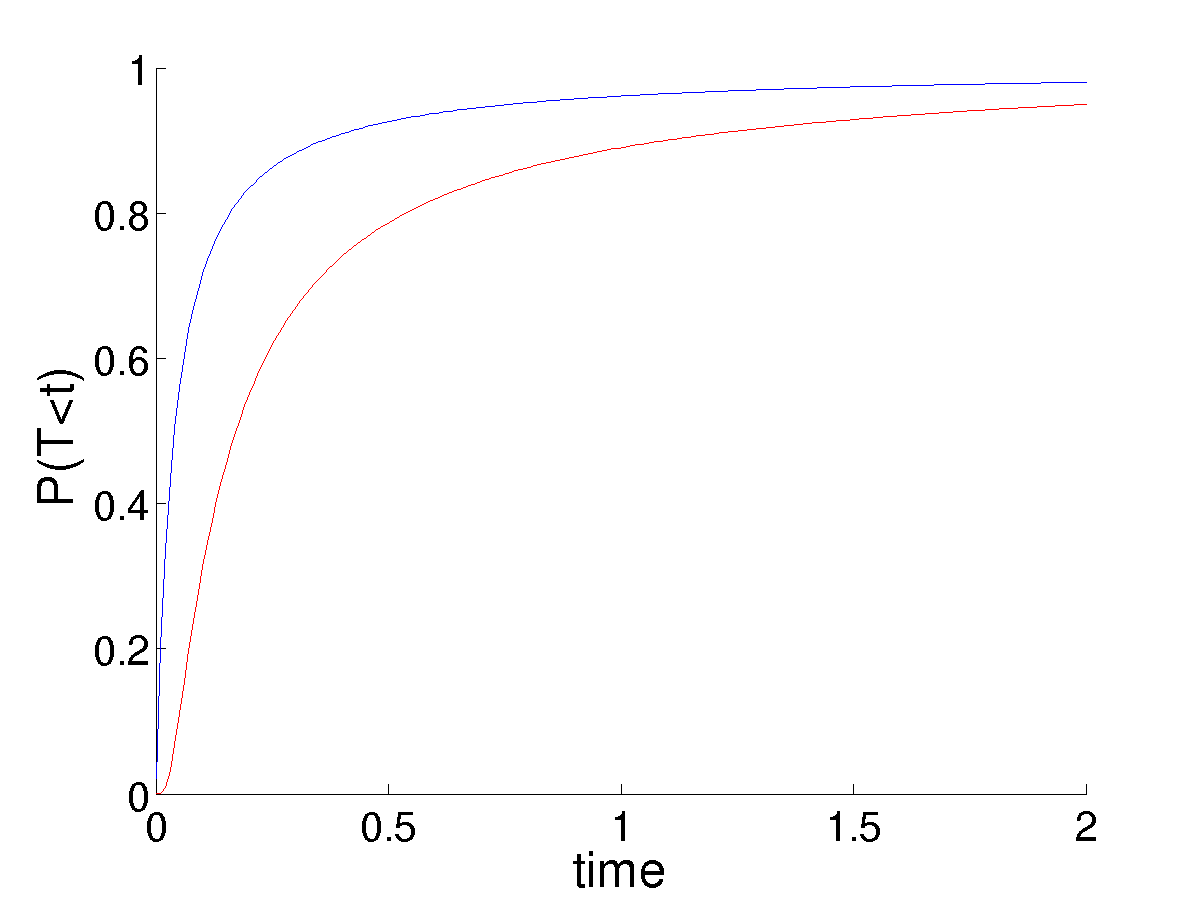
\includegraphics[width=\textwidth]{images/u}
\end{center}
\caption{Red line for dynamics of a population ten times smaller than that in the blue line}
\label{fig:u}
\end{figure}

\end{document}

If selection is strong relative to drift, we need only consider two steps for branching to occur successfully -- that a mutant occur in the coexistence region, $P_2$, and successfully survive the period when it is at low numbers.  The probability of a mutant with trait $y\in P_2$ occurring in a resident population with trait $x$ and surviving this initial vulnerable, low number state (surviving drift) has been described in our earlier writeup.  In this we used the branching process approach to determine the probability $u$ of surviving drift,
\begin{equation}
u=1-\frac{d}{b},
\label{branch}
\end{equation}
though we could equally well take the classical diffusion approach of Kimura,
\begin{equation}
u = \frac{1-e^{-2s}}{1-e^{-2sN}}; \qquad s = \frac{b-d}{b+d}.
\label{drift}
\end{equation}

Around the branching point, we are concerned with the phenomenon that a clone type, such as the initial resident, may face stochastic extinction even though its numbers are large.  

In particular, we are interested in the case when population is small enough and selection weak enough that the classical theory of density independent branching processes is not sufficient.  



We contrast this example to the case of a mutant introduced far from the branching point.  
\end{document}


